\documentclass[aspectratio=169,unicode,dvipdfmx,14pt]{beamer}

\usepackage{url}
\usepackage{bm}
\usepackage{amsmath}
\usepackage{amssymb}
\usepackage{graphicx}
\usepackage[absolute,overlay]{textpos}
\usepackage{hyperref}
\usepackage{listings}

\usefonttheme[onlymath]{serif}

\DeclareMathOperator*{\argmax}{argmax}

\hypersetup{
	setpagesize=false,
	bookmarksnumbered=true,%
	bookmarksopen=true,%
	colorlinks=true,%
	linkcolor=blue,
	citecolor=red,
}

\newcommand\FontMath{\fontsize{10}{12}\selectfont}
\renewcommand{\baselinestretch}{1.3}
\renewcommand{\familydefault}{\sfdefault}
\renewcommand{\kanjifamilydefault}{\gtdefault}
\usepackage[deluxe, expert]{otf}

\setbeamertemplate{navigation symbols}{}
\setbeamertemplate{footline}[frame number]
\setbeamerfont{footline}{size={\fontsize{15}{15}}}

\setbeamerfont{author}{size=\Large}
\setbeamerfont{institute}{size=\normalsize\itshape}
\setbeamerfont{title}{size=\huge}
\setbeamerfont{subtitle}{size=\LARGE\normalfont\slshape}


\title{ \\多項分布}
\author{\texorpdfstring{正田 備也\newline\href{mailto:masada@rikkyo.ac.jp}{masada@rikkyo.ac.jp}}{正田 備也}}
\date{}

\begin{document}

\begin{frame}
\titlepage
\end{frame}

\section{データのモデリング}

\begin{frame}\frametitle{Contents}
\Large \tableofcontents[currentsection]
\end{frame}

\begin{frame}{データのモデリング data modeling}
\begin{itemize}
\item この授業で扱うのは、統計モデルのうち、観測データが生成generateされる過程を数式で書くことで得られるモデル
\item このようなモデルを、生成モデルgenerative modelと呼ぶ
\begin{itemize}
\item 観測データがどのように生成されるかを考えないモデルを、識別モデルdiscriminative modelと呼ぶ
\end{itemize}
\item 観測データは、特定の確率分布にしたがって生成されるものとしてモデル化される
\item データを生成する分布のパラメータを推定することが、生成モデルを使った統計モデリングにおける課題となる
\end{itemize}
\end{frame}

\begin{frame}{観測変数}
\begin{itemize}
\item データは$n$回の観測の結果$\{x_1,x_2,\ldots,x_n\}$として表される
\item 各$x_i$は$i$番目の観測値を表す確率変数で、観測変数と呼ぶ
\begin{itemize}
\item[例1.] 同じ畑で獲れたトマトの重さ(連続量)
\item[例2.] 同じ文書に出現する単語(離散量)
\end{itemize}
\item 生成モデルを使うときは、各$x_i$がどのような値をとるかは特定の確率分布にしたがって確率的に決まると仮定する
\begin{itemize}
\item[例1.] 同じ畑で獲れたトマトの重さは同じ正規分布にしたがうと仮定
\item[例2.] 同じ文書に出現する単語は同じカテゴリカル分布にしたがうと仮定
\end{itemize}
\item 観測データが与えられているとき、その観測データを生成する確率分布を推定することが、生成的モデリングの課題
\end{itemize}
\end{frame}

\begin{frame}{独立同分布の仮定(i.i.d.の仮定)}
\begin{itemize}
\item $n$回の観測のそれぞれ$x_1,\ldots,x_n$が、同じ分布にしたがい、かつ、独立にしたがう、と仮定することが多い
\item 同じ分布にしたがうとは、例えば、単変量正規分布でモデリングする場合、$x_1,\ldots,x_n$の全てが同じ平均パラメータ$\mu$と標準偏差パラメータ$\sigma$をもつ正規分布にしたがうということ
\item 独立にしたがうとは、任意の$i$と$j$について、$x_i$がどの値をとるかは$x_j$がどの値をとるかに``左右されない''ということ
\begin{itemize}
\item 正確には、同時累積分布関数が周辺累積分布関数の積に一致する、ということ(つまり$P(x_i<a,x_j<b)=P(x_i<a)P(x_j<b)$)
\end{itemize}
\end{itemize}
\end{frame}


\begin{frame}{例1. 同じ畑で獲れたトマトの重さのモデル化}
\begin{itemize}
\item 同じ畑で獲れたトマトの重さは、独立に同じ正規分布にしたがうと仮定
\item 実際にある畑で獲れた327個の重さを測定したところ、$x_1=147, x_2=171, x_3=153, \ldots, x_{327}=144$だった(単位g)
\item これら測定値の平均は$156.4$、標準偏差は$20.8$だった
\item ということは、この畑から取れるトマトの重さは、平均が$156.4$で標準偏差が$20.8$の正規分布にしたがうだろう
\begin{itemize}
\item このように、統計モデリングでは、観測データをもとに、それを生成する確率モデルのパラメータを推定する
\begin{itemize}
\item ここで示したのは、最尤推定によるパラメータ推定
\end{itemize}
\end{itemize}
\end{itemize}
\end{frame}

\begin{frame}{例2. 同じ文書に出現する単語のモデル化}
\begin{itemize}
\item 同じ文書に出現する単語は、独立に同じカテゴリカル分布にしたがうと仮定
\item 実際に長さ4,503の文書に出現する単語を観測したところ、$x_1=\mbox{``this''}, x_2=\mbox{``is''}, \ldots, x_{4503}=\mbox{``pencil''}$だった
\item 各単語の出現回数を求めると``this''は23回、``is''は55回、``pencil''は8回、等々だった
\item ということは、この文書での単語の出現は、``this''の出現確率が$\frac{23}{4503}$、``is''の出現確率が$\frac{55}{4503}$、``pencil''の出現確率が$\frac{8}{4503}$、等々であるカテゴリカル分布にしたがうだろう
\begin{itemize}
\item これも、最尤推定によるパラメータ推定
\end{itemize}
\end{itemize}
\end{frame}


\begin{frame}{生成モデルの評価}
\begin{itemize}
\item まず、生成モデルのパラメータの値を推定しておく
\begin{itemize}
\item 最尤推定はパラメータ推定手法の一つ
\end{itemize}
\item そのパラメータの値を使って、未知データの確率を計算する
\item 計算された確率の``的確さ''で生成モデルの良し悪しを評価
\begin{itemize}
\item 未知データの確率の高低が、注目している事象に対応しているか
\begin{itemize}
\item 確率が高い=その生成モデルによって生成されそう
\item 確率が低い=その生成モデルによって生成されなさそう
\item 的確さ=注目している事象の起こりやすさに対応
\end{itemize}
\end{itemize}
\end{itemize}
\begin{textblock*}{0.4\linewidth}(285pt, 160pt)
    \centering
    
\includegraphics[width=0.5\linewidth]{kenkoushindan_ketsuatsu}
\end{textblock*}

\end{frame}

\begin{frame}{例. センサ測定値の統計モデル}
\begin{itemize}
\item 特定の環境におかれた特定のセンサの読み値の列が生成される過程を数式で書き、生成モデルを作る
\item この統計モデルのパラメータを推定する
\item 推定されたパラメータを使って、新たに得られた読み値の列が生成される確率を計算する
\item その環境におかれたそのセンサの読み値の列として大いにありうる読み値の列については高めの確率が得られ、
そうでない読み値の列については低めの確率が得られれば、良い統計モデルだと評価できるかもしれない
\end{itemize}
\end{frame}

\section{テキストデータのモデリング}

\begin{frame}\frametitle{Contents}
\Large \tableofcontents[currentsection]
\end{frame}

\begin{frame}{bag-of-wordsモデル}
\begin{itemize}
\item テキストデータのモデリングでは、よくbag-of-wordsモデルが使われる
\item bag-of-wordsモデルでは、単語の出現順序は考慮しない
\item つまり、単語の出現頻度だけを考慮して生成モデルを作る
\begin{itemize}
\item 語順を無視したテキストデータ分析でも、かなりのことが分かる
\end{itemize}
\item 言い換えれば、bag-of-wordsモデルでは、文書は単語のmultisetとしてモデル化される
\begin{itemize}
\item multisetとは、同じアイテムが重複して含まれることもある集合
\begin{itemize}
\item 通常の集合setは、要素はその集合に含まれるか含まれないかのどちらか
\end{itemize}
\item[例.]  買い物かごの中身
\end{itemize}
\end{itemize}
\end{frame}

\begin{frame}{例. 買い物かごの中身}
\begin{figure}[htbp]
\begin{center}
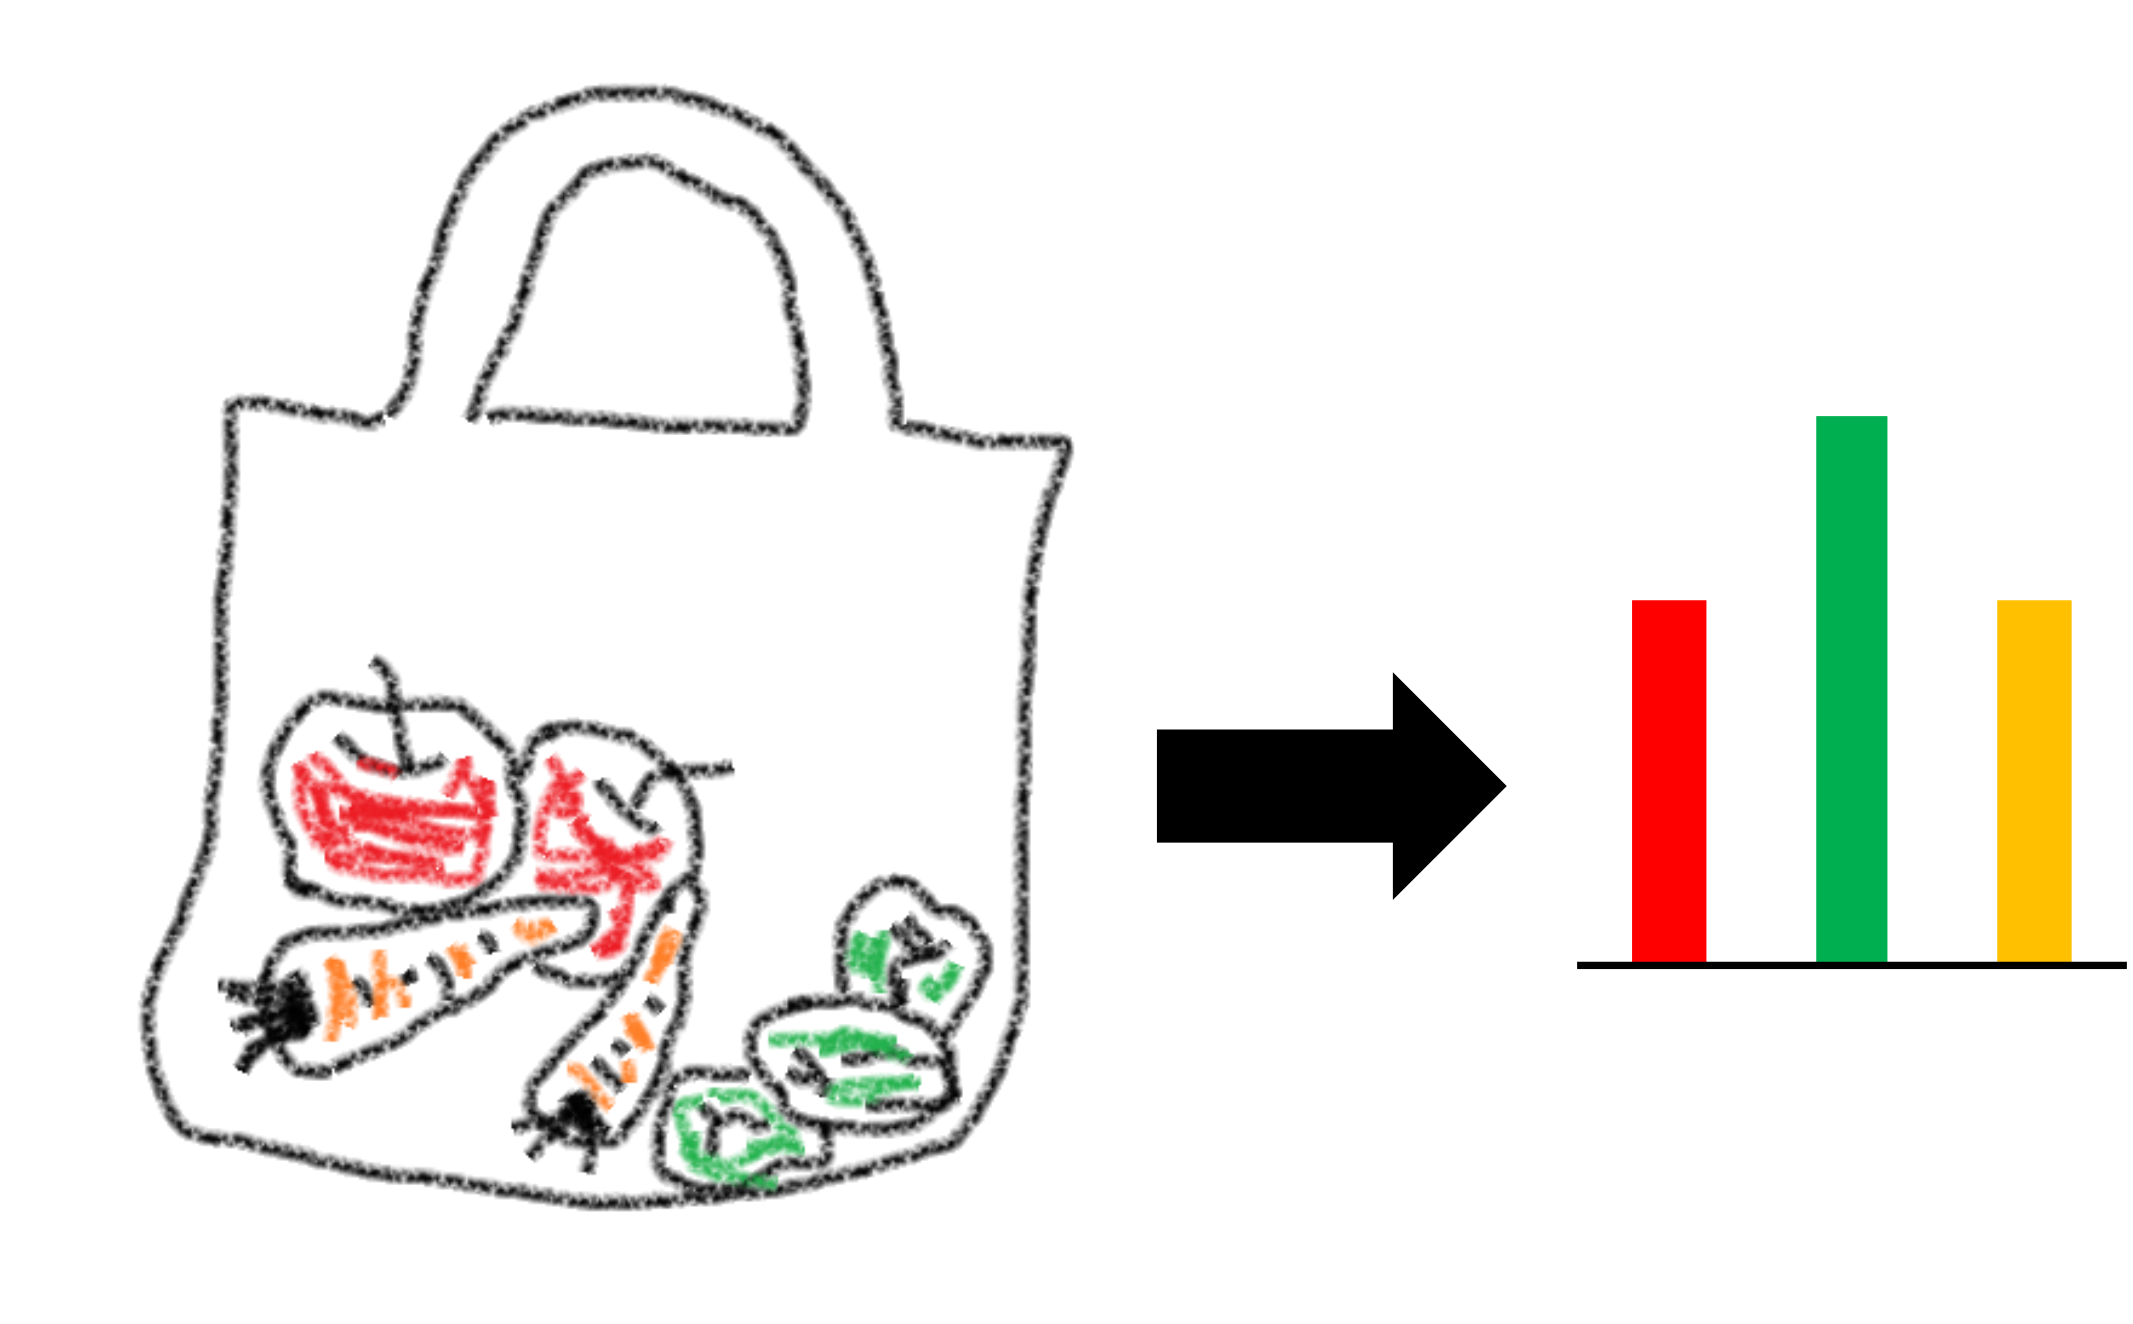
\includegraphics[scale=0.14]{bagofwords.png}
\label{}
\end{center}
\end{figure}
\end{frame}

\begin{frame}{出現頻度から確率へ}
\begin{itemize}
\item 各単語の出現頻度が分かっている
\begin{itemize}
\item 観測データ=各単語の出現頻度
\end{itemize}
\item これをもとに各単語の出現確率を求める
\begin{itemize}
\item どうすればいい?
\item[例.] 前のスライドで、リンゴの出現確率は?
\item モデルが違うと答えが違ってくる
\item $\mbox{リンゴの出現確率}=2/7$はひとつの答えにすぎない
\end{itemize}
\end{itemize}
\begin{textblock*}{0.4\linewidth}(300pt, 60pt)
    \centering
    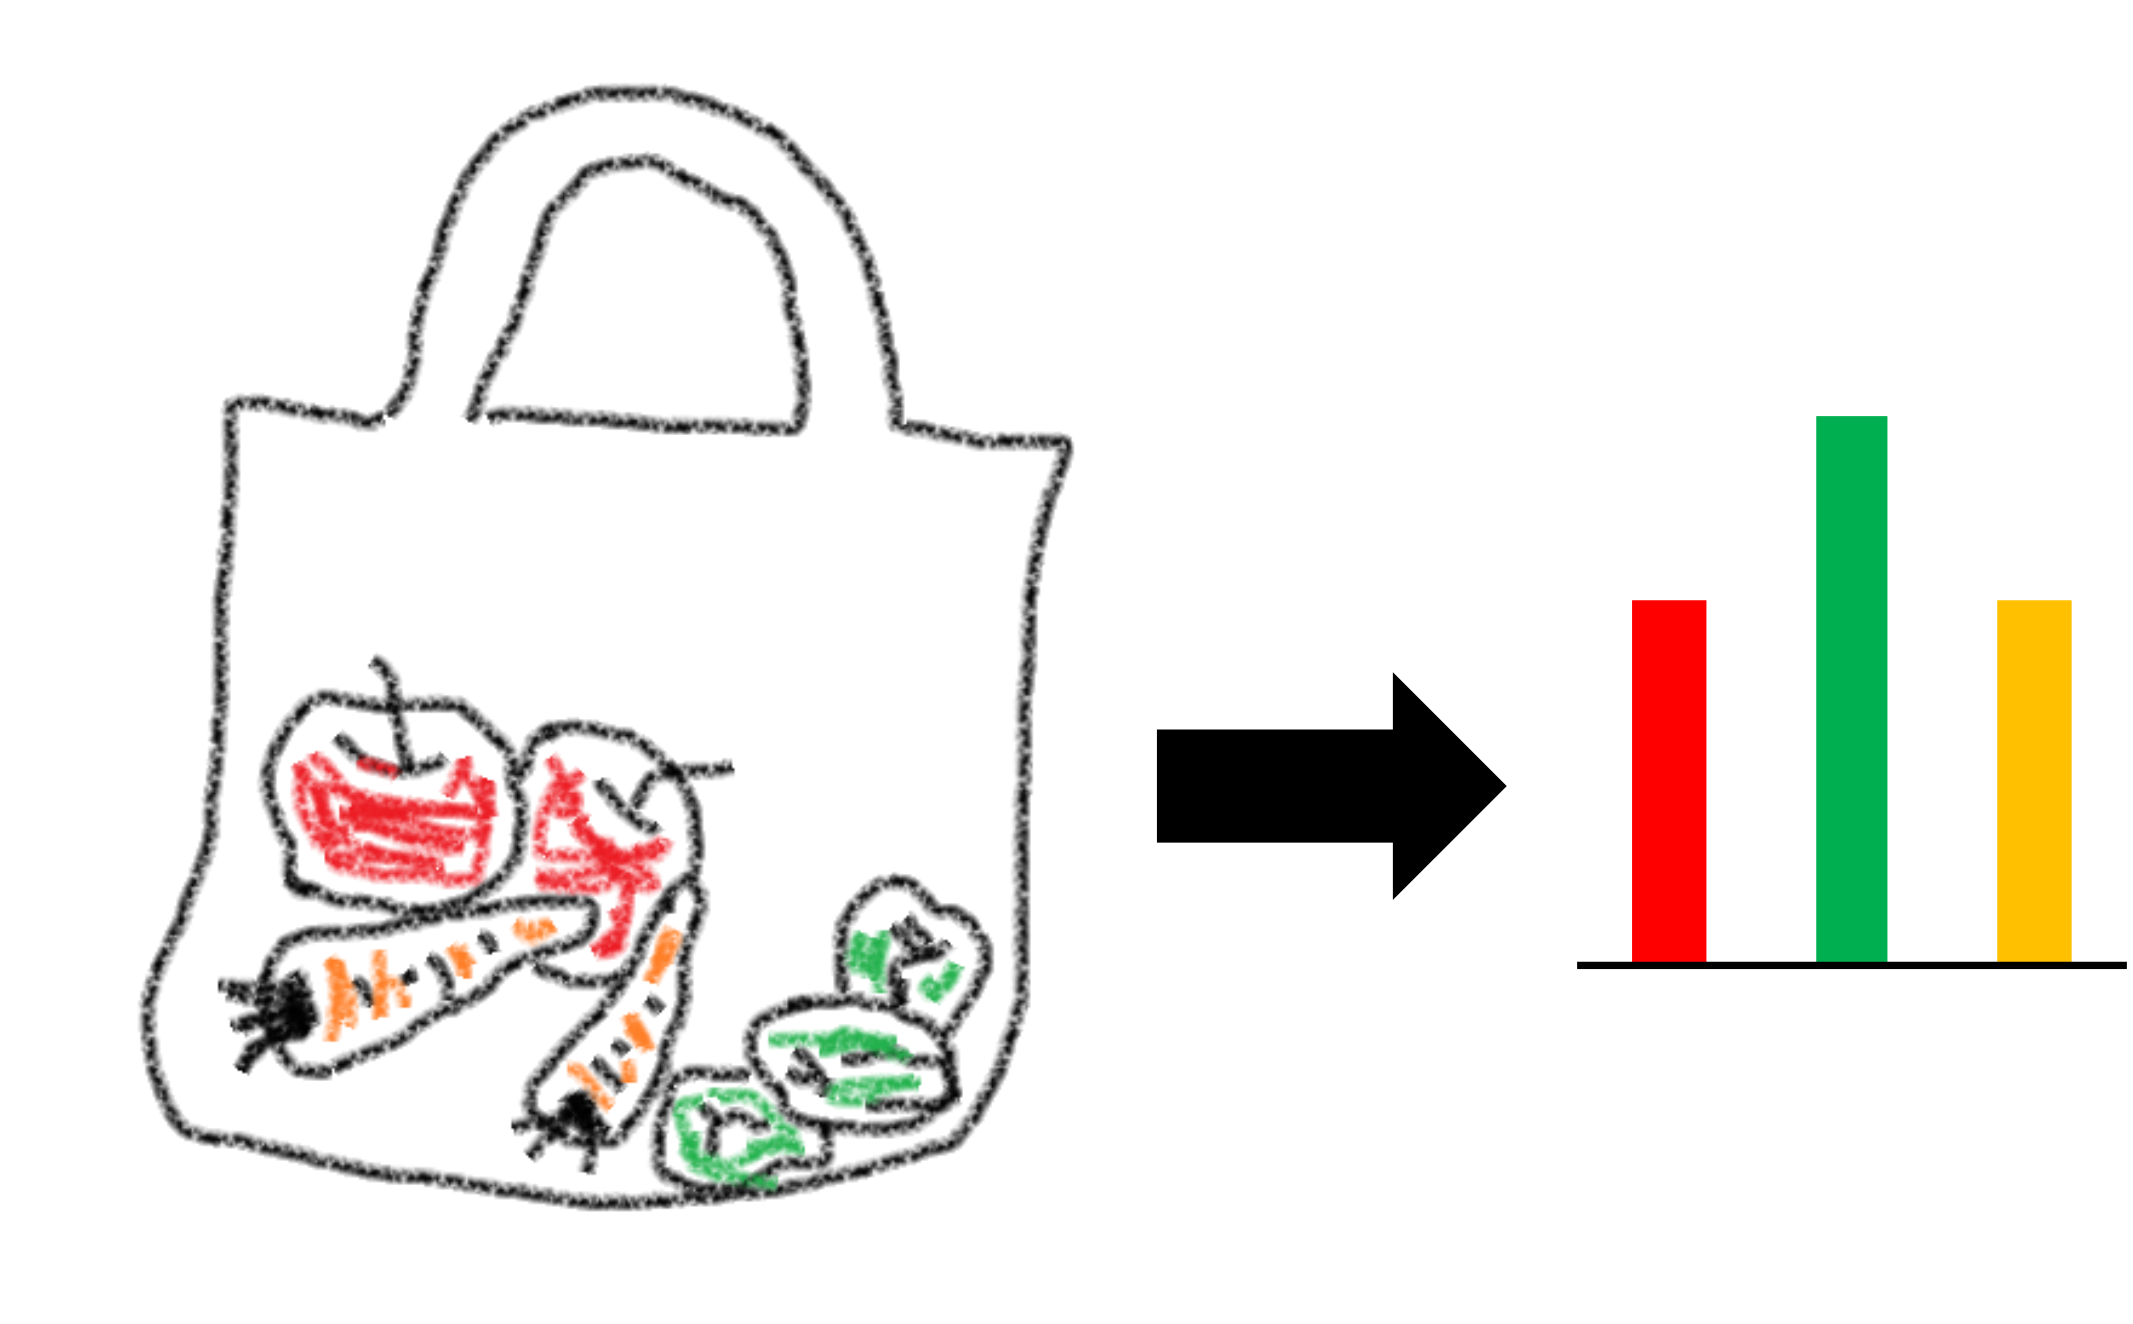
\includegraphics[width=.8\linewidth]{bagofwords.png}
\end{textblock*}
\end{frame}

\begin{frame}{bag-of-wordsではないモデル}
\begin{itemize}
\item $i$番目に出現する単語が何か、
つまり、$x_i$がどんな値をとるかが、それ以前にどんな単語が出現したかに依存して決まる、
つまり、$x_1,\ldots,x_{i-1}$という$i-1$個の確率変数の値に依存して決まるモデルは、
bag-of-wordsモデルではない
\item このように、それまでに出現した単語に依存して次の単語の出現確率が定まるモデルをautoregressiveモデルという
\begin{itemize}
\item 逆に言えば、bag-of-wordsモデルは$p(x_i|x_{i-1},\ldots,x_1)=p(x_i)$が成り立つことを仮定している
\end{itemize}
\item autoregressiveモデルも、最近はよく使われる
\end{itemize}
\end{frame}


\section{二項分布の復習}

\begin{frame}\frametitle{Contents}
\Large \tableofcontents[currentsection]
\end{frame}

\begin{frame}{ベルヌーイ分布 Bernoulli distribution}
\begin{itemize}
\item $V=\{\mbox{v}_1,\mbox{v}_2\}$という2種類のアイテムの集合上に定義される確率分布
\item パラメータは$\bm{\phi} = (\phi_1, \phi_2)$
\begin{itemize}
\item アイテム$\mbox{v}_1$が出現する確率$\phi_1$
\item アイテム$\mbox{v}_2$が出現する確率$\phi_2$
\item $\phi_1 + \phi_2=1$が成り立つので、自由度は1
\item[] \
\item[] \
\end{itemize}
\end{itemize}
\begin{textblock*}{0.4\linewidth}(290pt, 110pt)
    \centering
    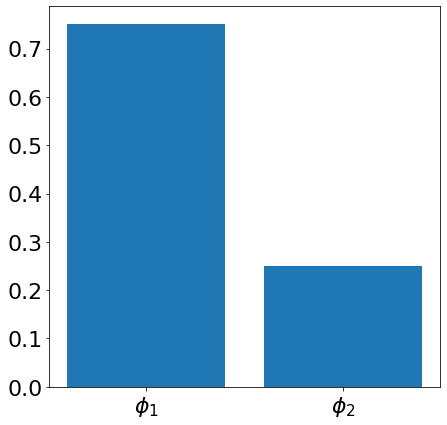
\includegraphics[width=0.8\linewidth]{bernoulli}
\end{textblock*}
\end{frame}

\begin{frame}{二項分布 binomial distribution}
\begin{itemize}
\item ベルヌーイ分布は1回のコイン投げのモデリングに使う
\item 複数回のコイン投げのモデリングには二項分布を使う
\item 試行回数を$n$として、$n$回のうち$\mbox{v}_1$が$k$回出現する確率がこれこれというふうに、$k=0$から$k=n$までのすべての場合に確率を割り振る確率分布が、二項分布
\item パラメータは$n$と$\bm{\phi} = (\phi_1, \phi_2)$
\begin{itemize}
\item 試行の回数$n$(これは観測データから決まる)
\item アイテム$\mbox{v}_1$が出現する確率$\phi_1$
\item アイテム$\mbox{v}_2$が出現する確率$\phi_2$
\item $\phi_1 + \phi_2=1$が成り立つので、自由度は1
\end{itemize}
\end{itemize}
\begin{textblock*}{0.4\linewidth}(305pt, 150pt)
    \centering
    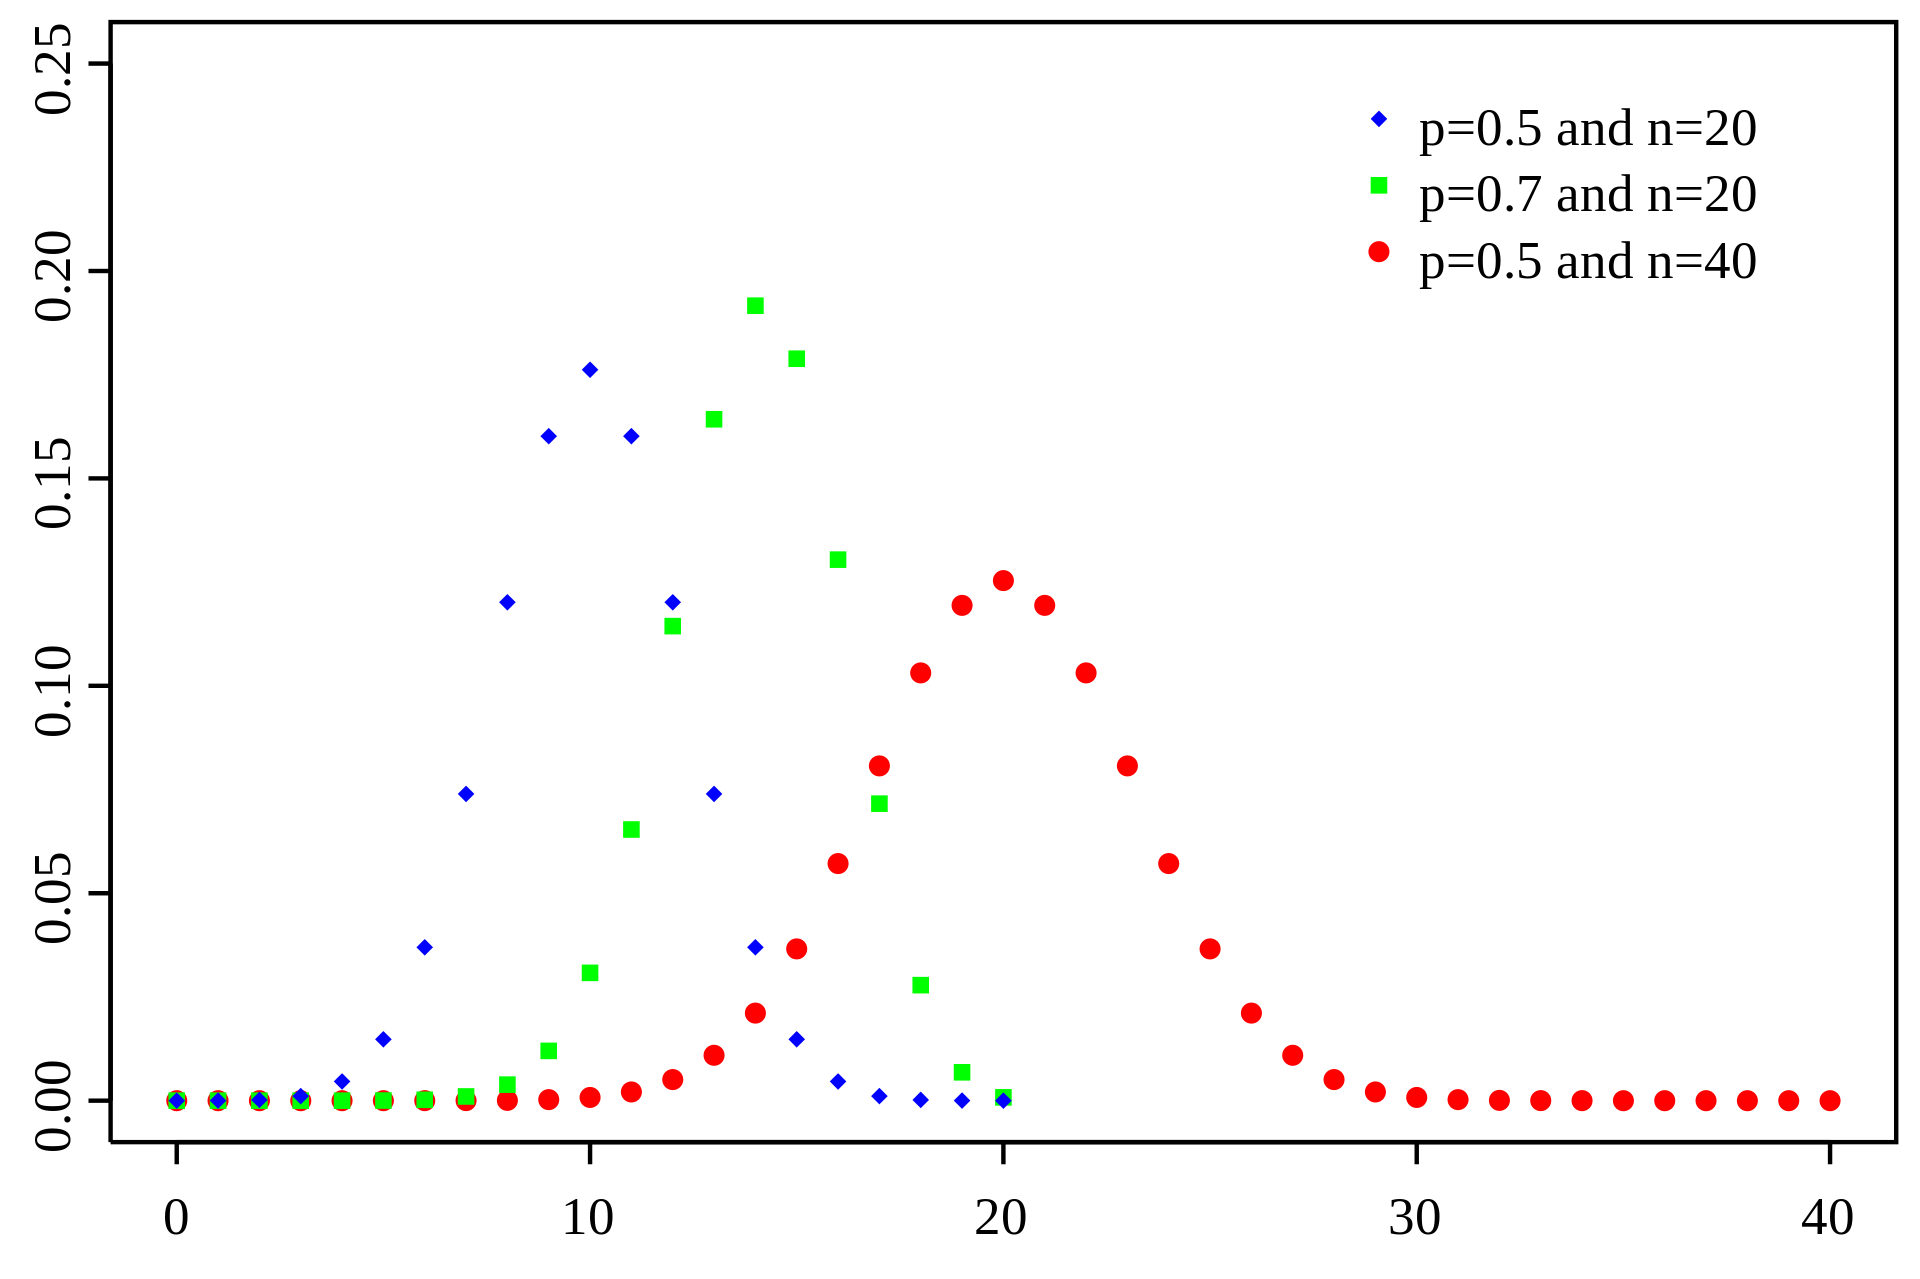
\includegraphics[width=0.8\linewidth]{1920px-Binomial_distribution_pmf.svg}
\end{textblock*}
\end{frame}

\begin{frame}
\begin{figure}[htbp]
\begin{center}
\vspace{.2in}
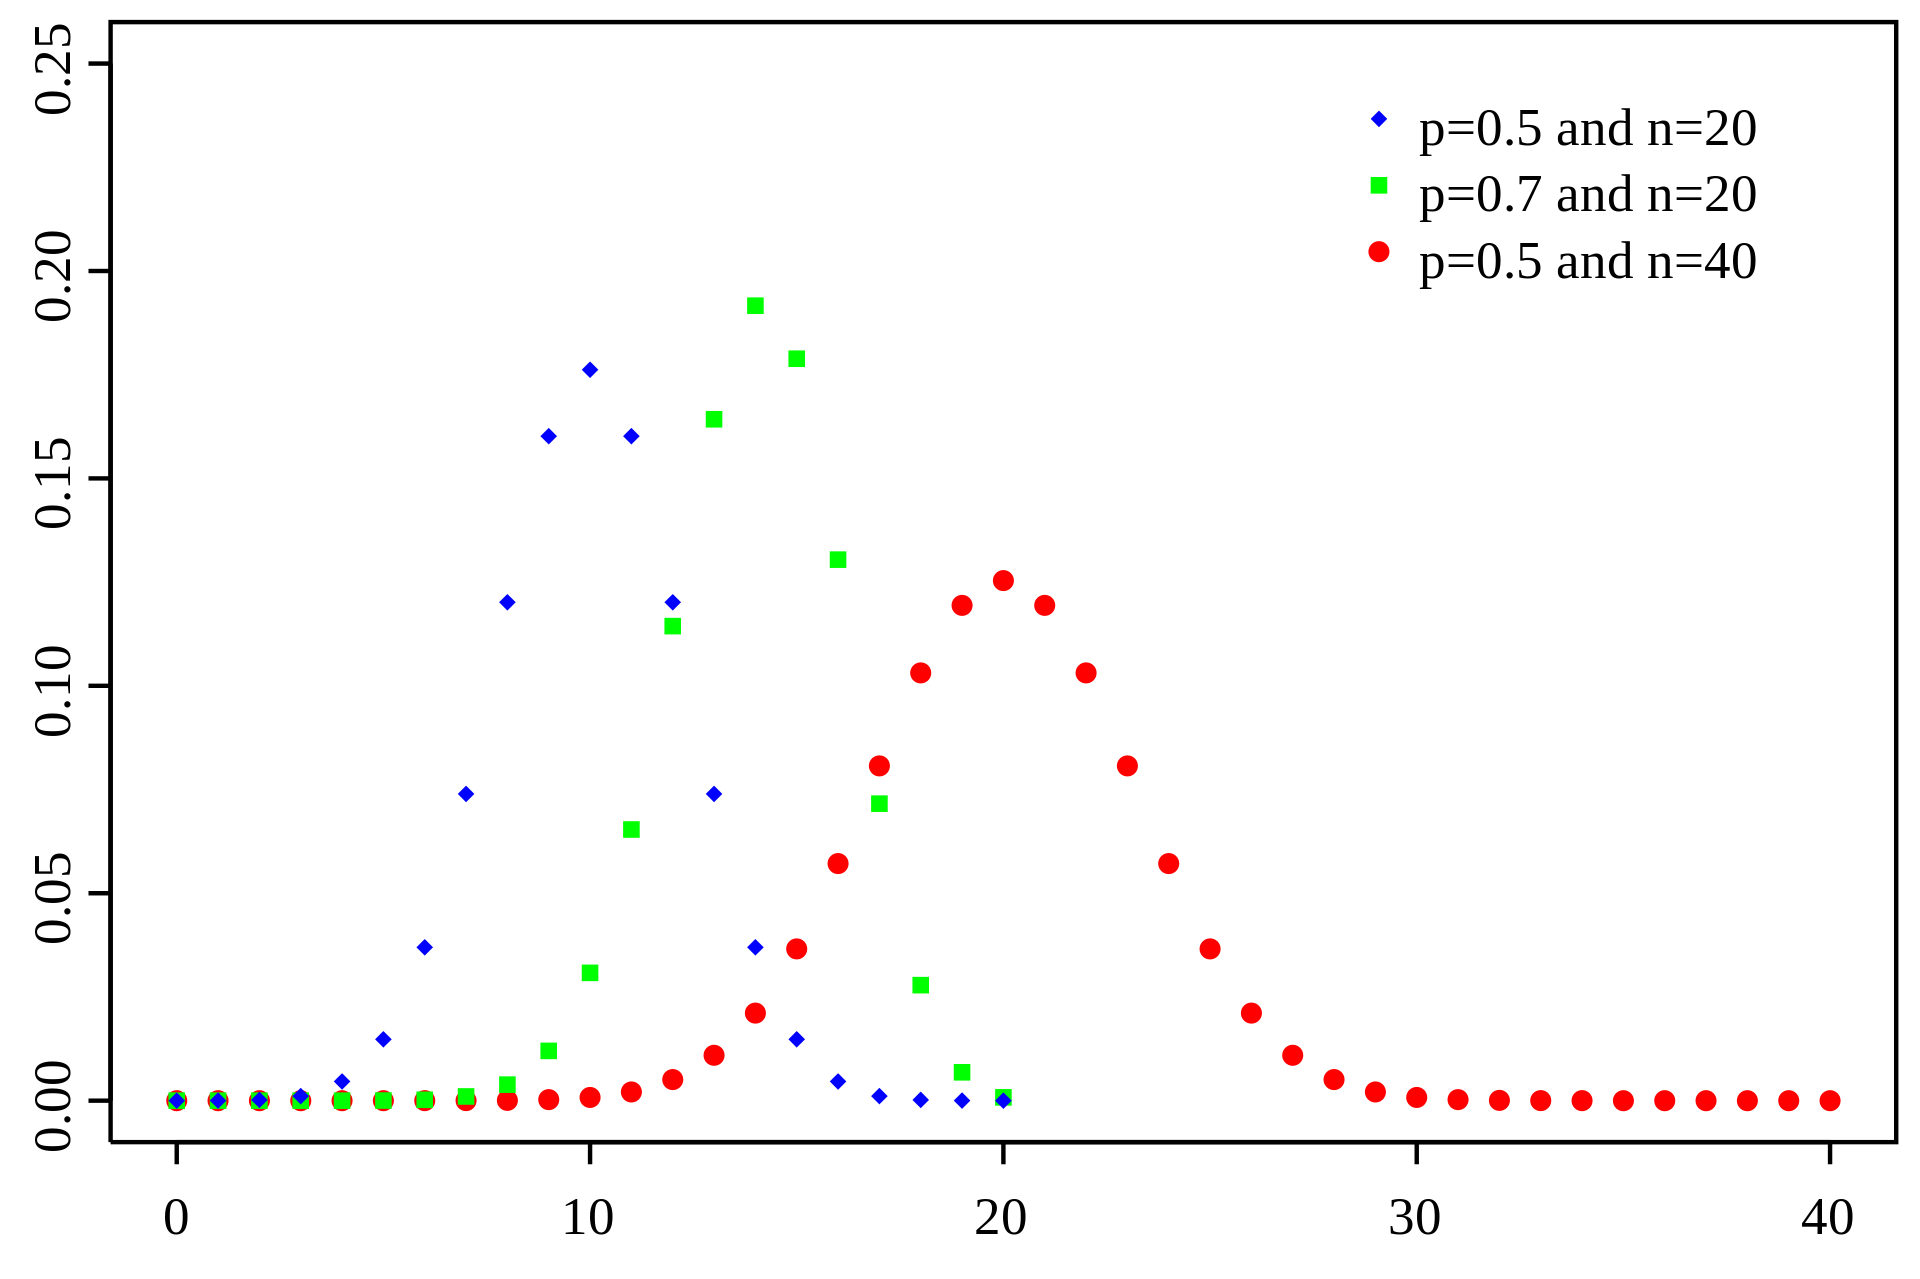
\includegraphics[scale=0.15]{1920px-Binomial_distribution_pmf.svg}
\caption{二項分布の確率質量関数の例}
\label{}
\end{center}
\end{figure}
\end{frame}

\begin{frame}{二項分布の確率質量関数}
\begin{itemize}
\item 確率質量関数 probability mass function; pmf
\begin{itemize}
\item 離散確率変数に、その値をとる確率を対応させる関数
\item 二項分布の場合は、表が出る回数にその確率を対応させる
\end{itemize}
\item 二項分布の確率質量関数
\begin{itemize}
\item $n$回の試行のうち$k$回$\mbox{v}_1$が出現する確率は:
\end{itemize}
\begin{align}
p(k;\bm{\phi},n)=\frac{n!}{k!(n-k)!}\phi_1^k\phi_2^{n-k}
\end{align}
\begin{itemize}
\item 「;」は、その右側にある$\phi_1$と$n$が自由パラメータ(我々が値を指定する必要があるパラメータ)であることを意味する
\end{itemize}
\end{itemize}
\end{frame}

\begin{frame}{二項分布の確率質量関数の読み方}
\begin{itemize}
\item[例.] コイン投げ
\begin{itemize}
\item $n$回の試行の列は$n$個の確率変数$x_1,\ldots,x_n$が表裏どちらの値をとるかで表される
(例:$x_1=\mbox{H},x_2=\mbox{H},\ldots,x_n=\mbox{T}$)
\item 各試行は、独立に同じベルヌーイ分布に従うと仮定
\item すると、表裏が出る順番に関係なく、表が$k$回、裏が$n-k$回出る試行の列の確率は
$\phi_1^k \phi_2^{n-k}$
\item つまり、表裏の出る順番が違うだけの試行の列を、二項分布によって区別してモデル化することはできない
(頻度が同じなら同じ)
\item よって、表$k$回、裏$n-k$回が出る試行の列一つ一つの確率は$\phi_1^k \phi_2^{n-k}$であっても、
二項分布のpmfは
$p(k;\bm{\phi},n)=\frac{n!}{k!(n-k)!}\phi_1^k\phi_2^{n-k}$
\end{itemize}
\end{itemize}
\end{frame}


\section{多項分布}

\begin{frame}\frametitle{Contents}
\Large \tableofcontents[currentsection]
\end{frame}

\begin{frame}{カテゴリカル分布}
\begin{itemize}
\item $V=\{\mbox{v}_1,\ldots,\mbox{v}_W\}$を$W$種類のアイテムの集合とする
\begin{itemize}
\item[例1.] サイコロの目($W=6$)
\item[例2.] 自然言語の語彙($W=\mbox{数千〜数十万}$)
\end{itemize}
\item カテゴリカル分布は$V$上に定義された離散確率分布
\item パラメータは$\bm{\phi}=(\phi_1,\ldots,\phi_W)$
\begin{itemize}
\item アイテム$\mbox{v}_w$が出現する確率$\phi_w$
\item $\sum_{w=1}^W \phi_w = 1$を満たす
\item[] \ 
\item[] \ 
\end{itemize}
\end{itemize}
\begin{textblock*}{0.5\linewidth}(230pt, 150pt)
    \centering
    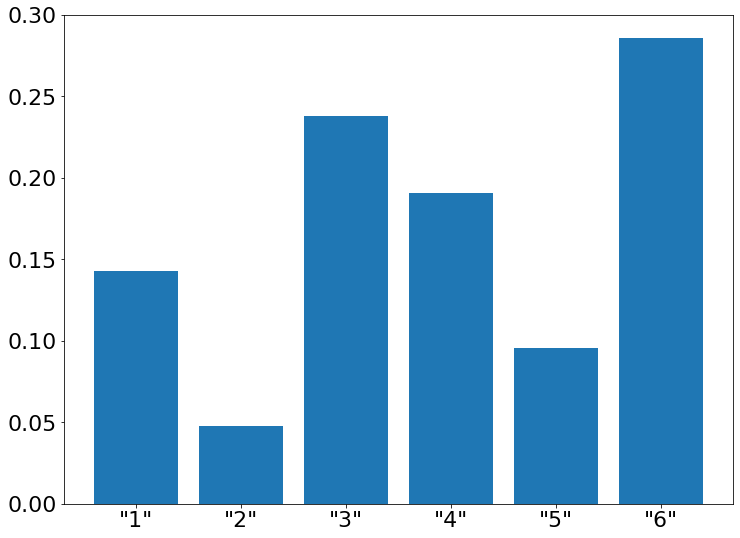
\includegraphics[width=0.7\linewidth]{dice_bar_chart.png}
\end{textblock*}
\end{frame}


\begin{frame}{多項分布 multinomial distribution}
\begin{itemize}
\item カテゴリカル分布は、1回の試行のモデリングに使う
\item 複数回の独立な試行のモデリングには、多項分布を使う
\item 計$n$回の試行のうち各アイテムが何回ずつ出現するか、その可能なすべての場合に確率を割り振る確率分布が多項分布
\begin{itemize}
\item 次のスライド参照
\end{itemize}
\item パラメータは$n$と$\bm{\phi}=(\phi_1,\ldots,\phi_W)$
\begin{itemize}
\item 試行の回数$n$(観測データから決まる)
\item アイテム$\mbox{v}_w$の出現確率$\phi_w$($\sum_w \phi_w = 1$を満たす)
\item $\sum_w \phi_w=1$が満たされるので、自由度は$W-1$
\end{itemize}
\end{itemize}
\end{frame}

\begin{frame}{多項分布はどのような集合の上に定義されるか}
\begin{itemize}
\item カテゴリカル分布はアイテムの集合の上に定義される
\begin{itemize}
\item すべてのアイテムにわたって確率を合計すると$1$になる
\end{itemize}
\item 多項分布は``計$n$回の試行のうち各アイテムが何回ずつ出現するかの、可能な全ての場合の集合''の上に定義される
\begin{itemize}
\item 多項分布は、各アイテムの出現回数が同じで、出現順が違うだけの試行列を区別できない
\item $W$種類のアイテムから重複を許して$n$個を選ぶすべての場合にわたって確率を合計すると1になる
\begin{itemize}
\item $W$種類のアイテムから重複を許して$n$個を選ぶ場合の数はいくら?
\item $n$個の「◯」と$W-1$個の「|」(仕切り)を並べる場合の数と同じ
\item[例.] 「◯ ◯ || ◯ | ◯ ◯ ◯ 」は、$n=6$で、$\mbox{v}_1$が2回、$\mbox{v}_2$が0回、$\mbox{v}_3$が1回、$\mbox{v}_4$が3回、それぞれ出現する場合を表す
\end{itemize}
\end{itemize}
\end{itemize}
\end{frame}

\begin{frame}{多項分布の確率質量関数}
\begin{itemize}
\item アイテム$\mbox{v}_w$の出現回数を$c_w$と書くことにする
\item 総試行回数を$n$とすると、当然$\sum_w c_w = n$が成り立つ
\item このとき、多項分布の確率質量関数pmfは以下ように書ける
\begin{align}
p((c_1,\ldots,c_W);\bm{\phi},n) = \frac{n!}{\prod_w c_w!}\prod_w\phi_w^{c_w}
\end{align}
\begin{itemize}
\item $\frac{n!}{\prod_w c_w!}$の部分は、$n$回の試行のうちアイテム$\mbox{v}_w$が$c_w$回出現するような試行の列の総数をあらわしている
\item 多項分布は、各アイテムの出現回数が同じで、出現順が違うだけの試行列を区別できない
\end{itemize}
\end{itemize}
\end{frame}

\section{多項分布の最尤推定}

\begin{frame}\frametitle{Contents}
\Large \tableofcontents[currentsection]
\end{frame}

\begin{frame}{多項分布によるモデリングに登場する変数}
\begin{itemize}
\item アイテムの出現列を表す観測変数$\bm{x}=\{x_1,\ldots,x_n\}$
\begin{itemize}
\item $x_i$は、$i$番目に出現したアイテムを表す\underline{確率変数}
\item[例.] $x_i = \mbox{``apple''}$は「$i$番目に出現する単語は``apple''」という意味
\item 観測変数なので、値はすでに与えられている(値が既知の変数)
\end{itemize}
\item 多項分布のパラメータ$\bm{\phi}=(\phi_1,\ldots,\phi_W)$
\begin{itemize}
\item $\phi_w$は、アイテム$\mbox{v}_w$の出現確率を表す\underline{パラメータ}
\item[例.] $\phi_w=0.0013$は「単語$\mbox{v}_w$の出現確率が$0.0013$」という意味
\item $\phi_w$は値が未知の変数
\item この値の推定が、多項分布によるモデリングにおいて解くべき問題
\end{itemize}
\end{itemize}
\end{frame}

\begin{frame}{多項分布の最尤推定}
\begin{itemize}
\item 観測データ$\bm{x}=\{x_1,\ldots,x_n\}$はアイテムの出現の列
\item 多項分布によるモデリングでは、出現順序は無視される
\item つまり、各アイテム$\mbox{v}_w$の出現回数$c_w$だけが問題とされる
\item このとき、観測データ$\bm{x}$の尤度は、$\bm{\phi}$の関数として、以下のように書ける
\begin{align}
p(\bm{x};\bm{\phi},n)=\frac{n!}{\prod_{w=1}^W c_w!}\prod_{w=1}^W\phi_w^{c_w}
\end{align}
\item 尤度を最大化する$\bm{\phi}$の値を推定値とするのが最尤推定
\begin{itemize}
\item 最尤推定のほかにも$\bm{\phi}$の値を推定する方法はある
\end{itemize}
\end{itemize}
\end{frame}

\begin{frame}{問題3-1}
\begin{itemize} 
\item 観測データ$\bm{c}=(c_1,\ldots,c_W)$の尤度
\begin{align}
p(\bm{x};\bm{\phi},n)=\frac{n!}{\prod_{w=1}^W c_w!}\prod_{w=1}^W\phi_w^{c_w} \notag
\end{align}
を最大化する$\bm{\phi}$を求めよう
\begin{itemize}
\item ヒント:ラグランジュの未定乗数法を使う(使わなくても解ける) 
\end{itemize}
\end{itemize}
\end{frame}

\begin{frame}{対数尤度の最大化}
\begin{itemize}
\item 多くの場合、尤度そのものではなく対数尤度を最大化する
\item 答えは同じだが、計算はしやすい
\end{itemize}
\begin{align}
\ln p(\bm{x};\bm{\phi},n)=\sum_{w=1}^W c_w\ln\phi_w + const.
\end{align}
\end{frame}

\begin{frame}
\FontMath
\begin{align}
L(\bm{\phi}) & = \ln p(\bm{x};\bm{\phi},n) + \lambda \Big( 1 - \sum_{w=1}^W \phi_w \Big)
\notag \\
& = \sum_{w=1}^W c_w\ln\phi_w  + \lambda \Big( 1 - \sum_{w=1}^W \phi_w \Big) + const.
\end{align}
とおく。
\begin{align}
\frac{\partial L(\bm{\phi})}{\partial \phi_w} & = \frac{c_w}{\phi_w} - \lambda \\
\frac{\partial L(\bm{\phi})}{\partial \lambda} & = 1 - \sum_{w=1}^W \phi_w
\end{align}

$\frac{\partial L(\bm{\phi})}{\partial \phi_w} = 0$より$\phi_w = \frac{c_w}{\lambda}$であり、
$\frac{\partial L(\bm{\phi})}{\partial \lambda} = 0$より$\sum_w \frac{c_w}{\lambda} = 1$である。

よって、$\lambda = \sum_w c_w$となり、$\phi_w = \frac{c_w}{\sum_{w^\prime} c_{w^\prime}}$を得る。
\end{frame}

\begin{frame}{多項分布の最尤推定の答え}
\begin{align}
\phi_w = \frac{c_w}{\sum_{w^\prime} c_{w^\prime}}
\end{align}
\begin{itemize}
\item 「当たり前では?」と思ってしまうのは、良くないかも
\item これはあくまで、ひとつの答え
\item 総出現回数$n$回のうち各アイテム$\mbox{v}_w$が$c_w$回ずつ出現しているデータをもとに、各アイテム$\mbox{v}_w$の出現確率$\phi_w$を推定する方法は、他にもある
\end{itemize}
\end{frame}

\section{多項分布の最尤推定の応用}

\begin{frame}\frametitle{Contents}
\Large \tableofcontents[currentsection]
\end{frame}

\begin{frame}{情報検索 information retrieval}
\begin{itemize}
\item たくさんの文書を持っている
\item それらの文書をクエリに適合する(relevantな)順にソート
\begin{itemize}
\item 情報検索とは、このようなことをすること
\end{itemize}
\item どう実装すればいい?
\item 実装例
\begin{itemize}
\item ひとつひとつの文書について別々に単語出現確率$\bm{\phi}$を最尤推定
\item 推定された$\bm{\phi}$を使って、クエリの生成確率を計算
\item この生成確率を高くする順に文書をソート
\end{itemize}
\end{itemize}
\end{frame}

\begin{frame}{文書をランキングするための計算}
\begin{itemize}
\item 上述の最尤推定は、検索対象の文書群のうち$d$番目の文書について単語$\mbox{v}_w$の出現確率を
$\hat{\phi}_{d,w} = \frac{c_{d,w}}{\sum_w n_d}$と与える
\item この単語確率によってクエリ$\bm{x}_q$が生成される確率は:
\begin{align}
p(\bm{x}_q | \hat{\bm{\phi}}_d) = \frac{n_q!}{\prod_w c_{q,w}!} \prod_w \bigg( \frac{c_{d,w}}{n_d} \bigg)^{c_{q,w}}
\end{align}
\begin{itemize}
\item $c_{q,w}$はクエリにおける単語$\mbox{v}_w$の出現頻度
\end{itemize}
\item $p(\bm{x}_q | \hat{\bm{\phi}}_d)$の降順に、文書をソートすればよい
\end{itemize}
\end{frame}

\begin{frame}
\begin{figure}[htbp]
\begin{center}
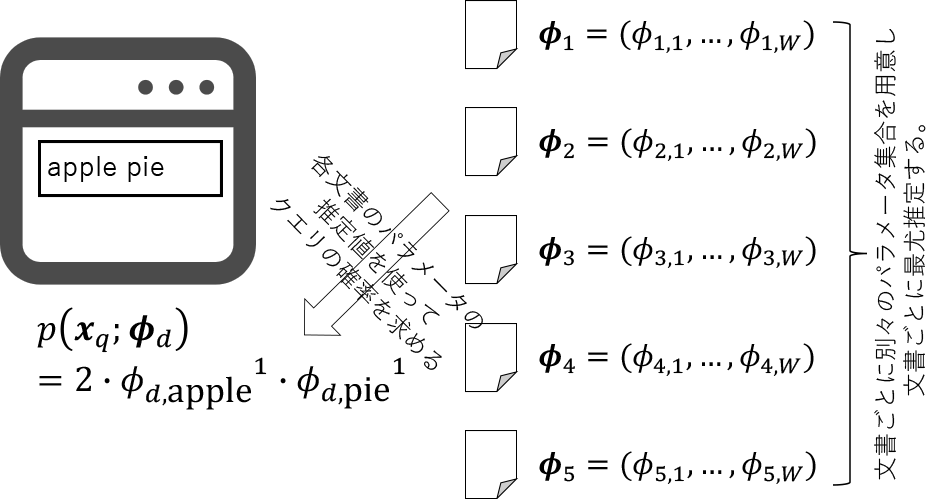
\includegraphics[scale=0.42]{information_retrieval.png}
\label{}
\end{center}
\end{figure}
\end{frame}


\end{document}